The objective of the experiment is to measure the $d'$ of a holographic grating using a second holographic grating with a known $d$. To do this I decided to study three different sources and try to use different methods. The values obtained are qualitatively consistent with each other even if they come from different configurations. During the data taking process I encountered some problems in quantifying the errors associated with direct measurements. In view of this, the goal has been achieved.
\newpage
\appendix
\section{Images taken without wide-angle}
\begin{figure}[htp!]
  \centering
  
\includegraphics[scale=0.07]{Conclusione/gg.png} 
  \centering
  \qquad 
\includegraphics[scale=0.07]{Conclusione/ff.png}
  \caption{These two images have been taken without wide angle.}
\end{figure}
\section{Measurement Methods}
Here are some images taken during the measurement of $ \Delta x $ using the Imagej software:
\begin{figure}[htp!]
  \centering
  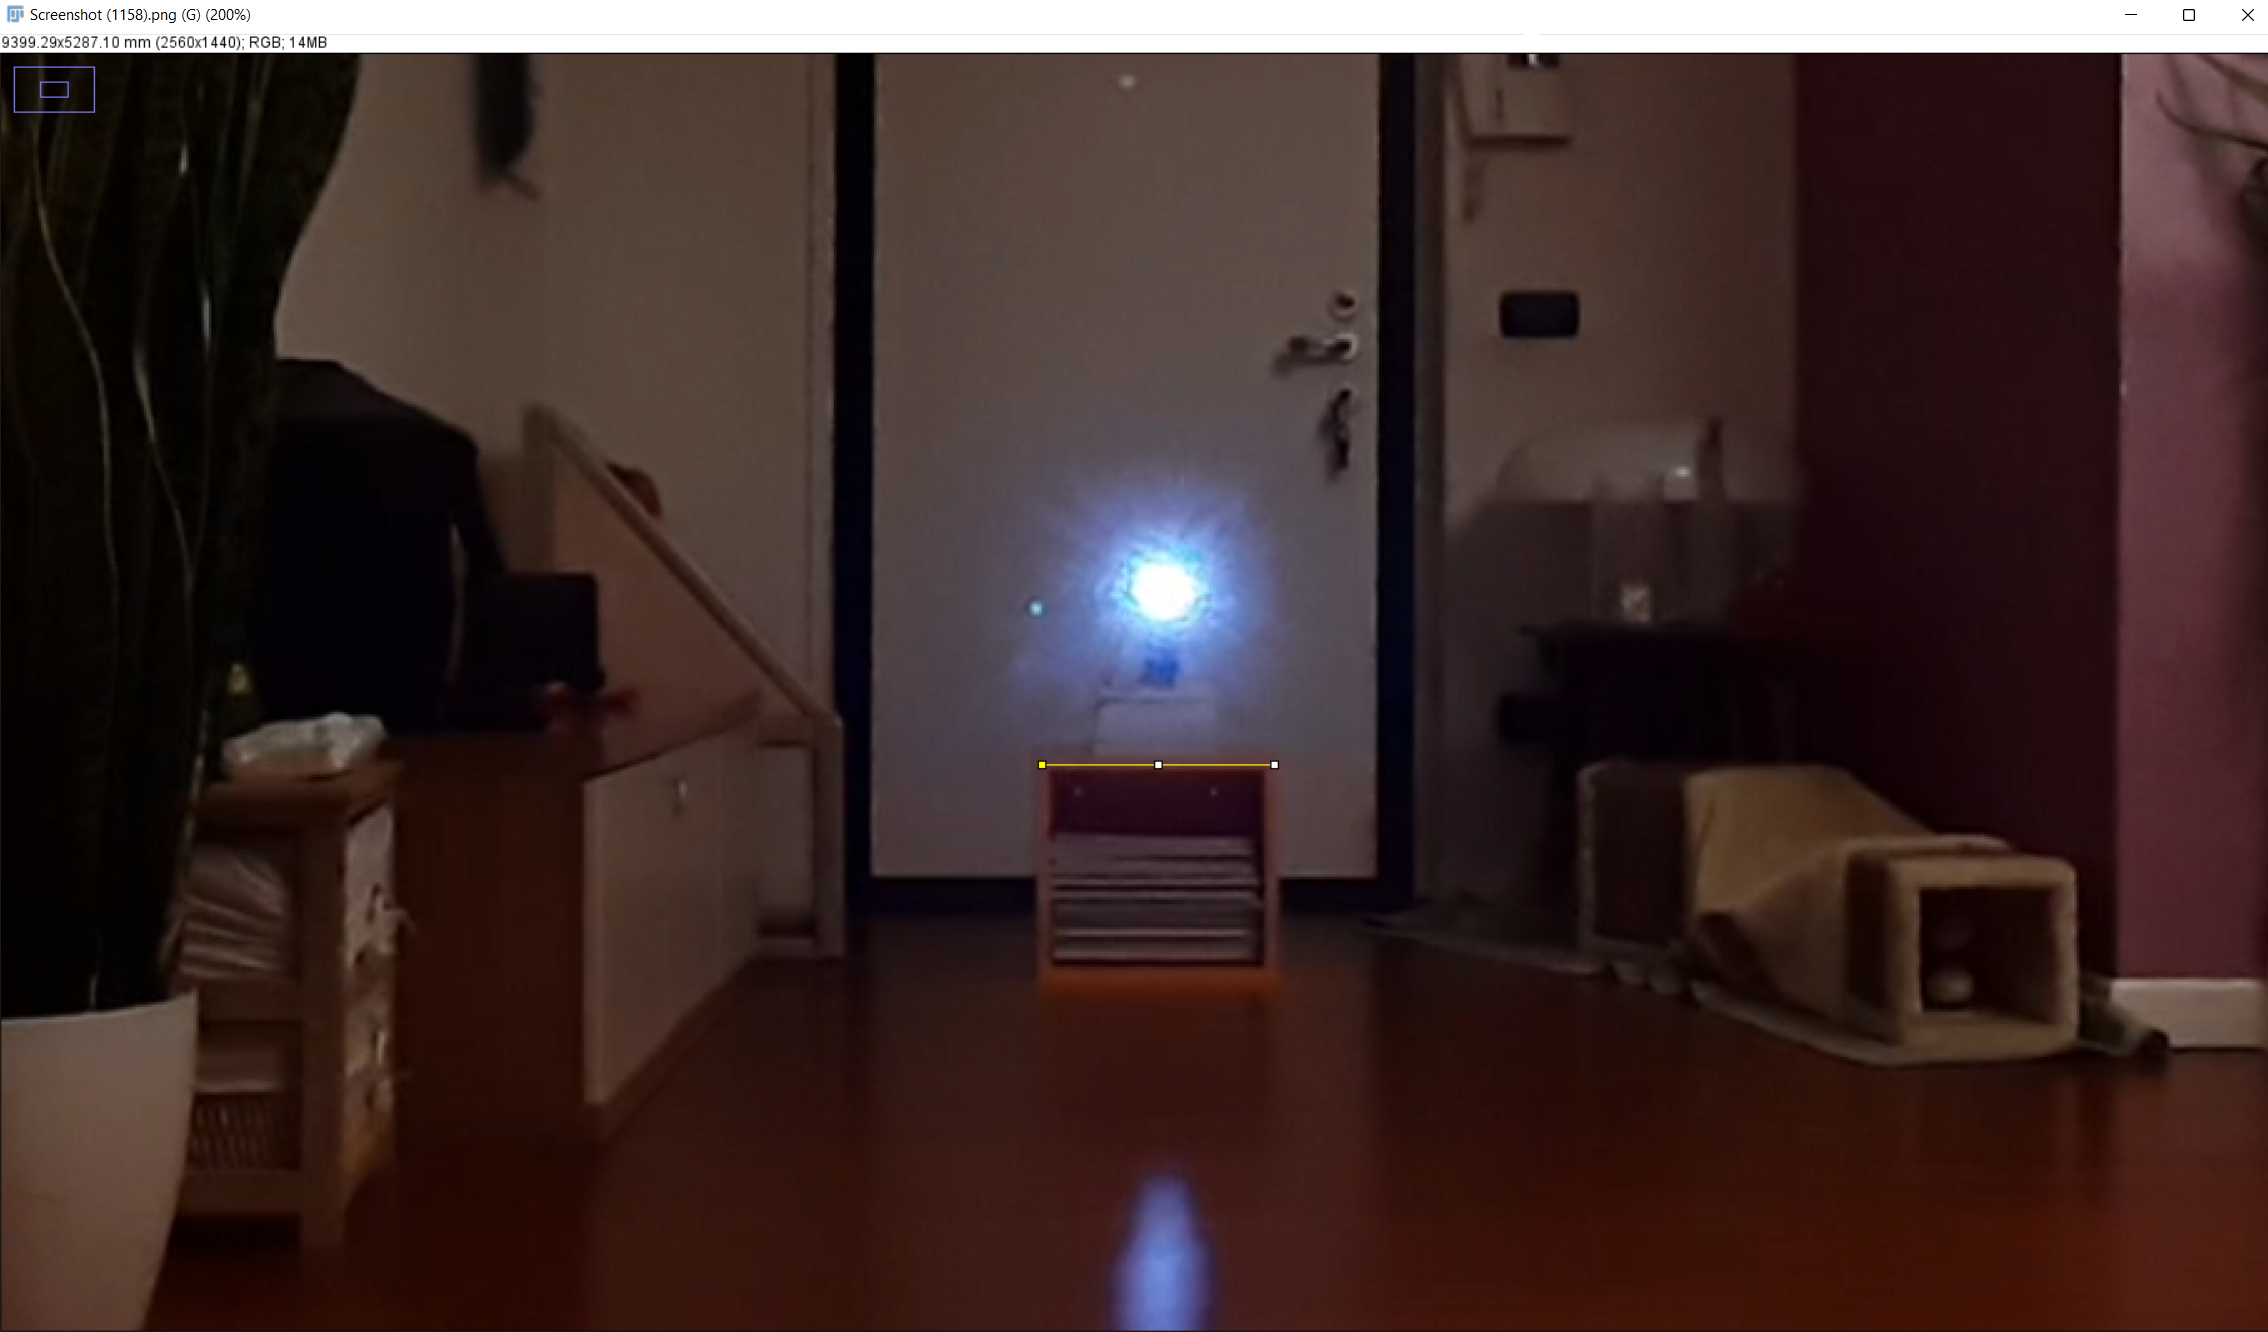
\includegraphics[scale=0.15]{Conclusione/Sist.png} 
  \centering
  \qquad 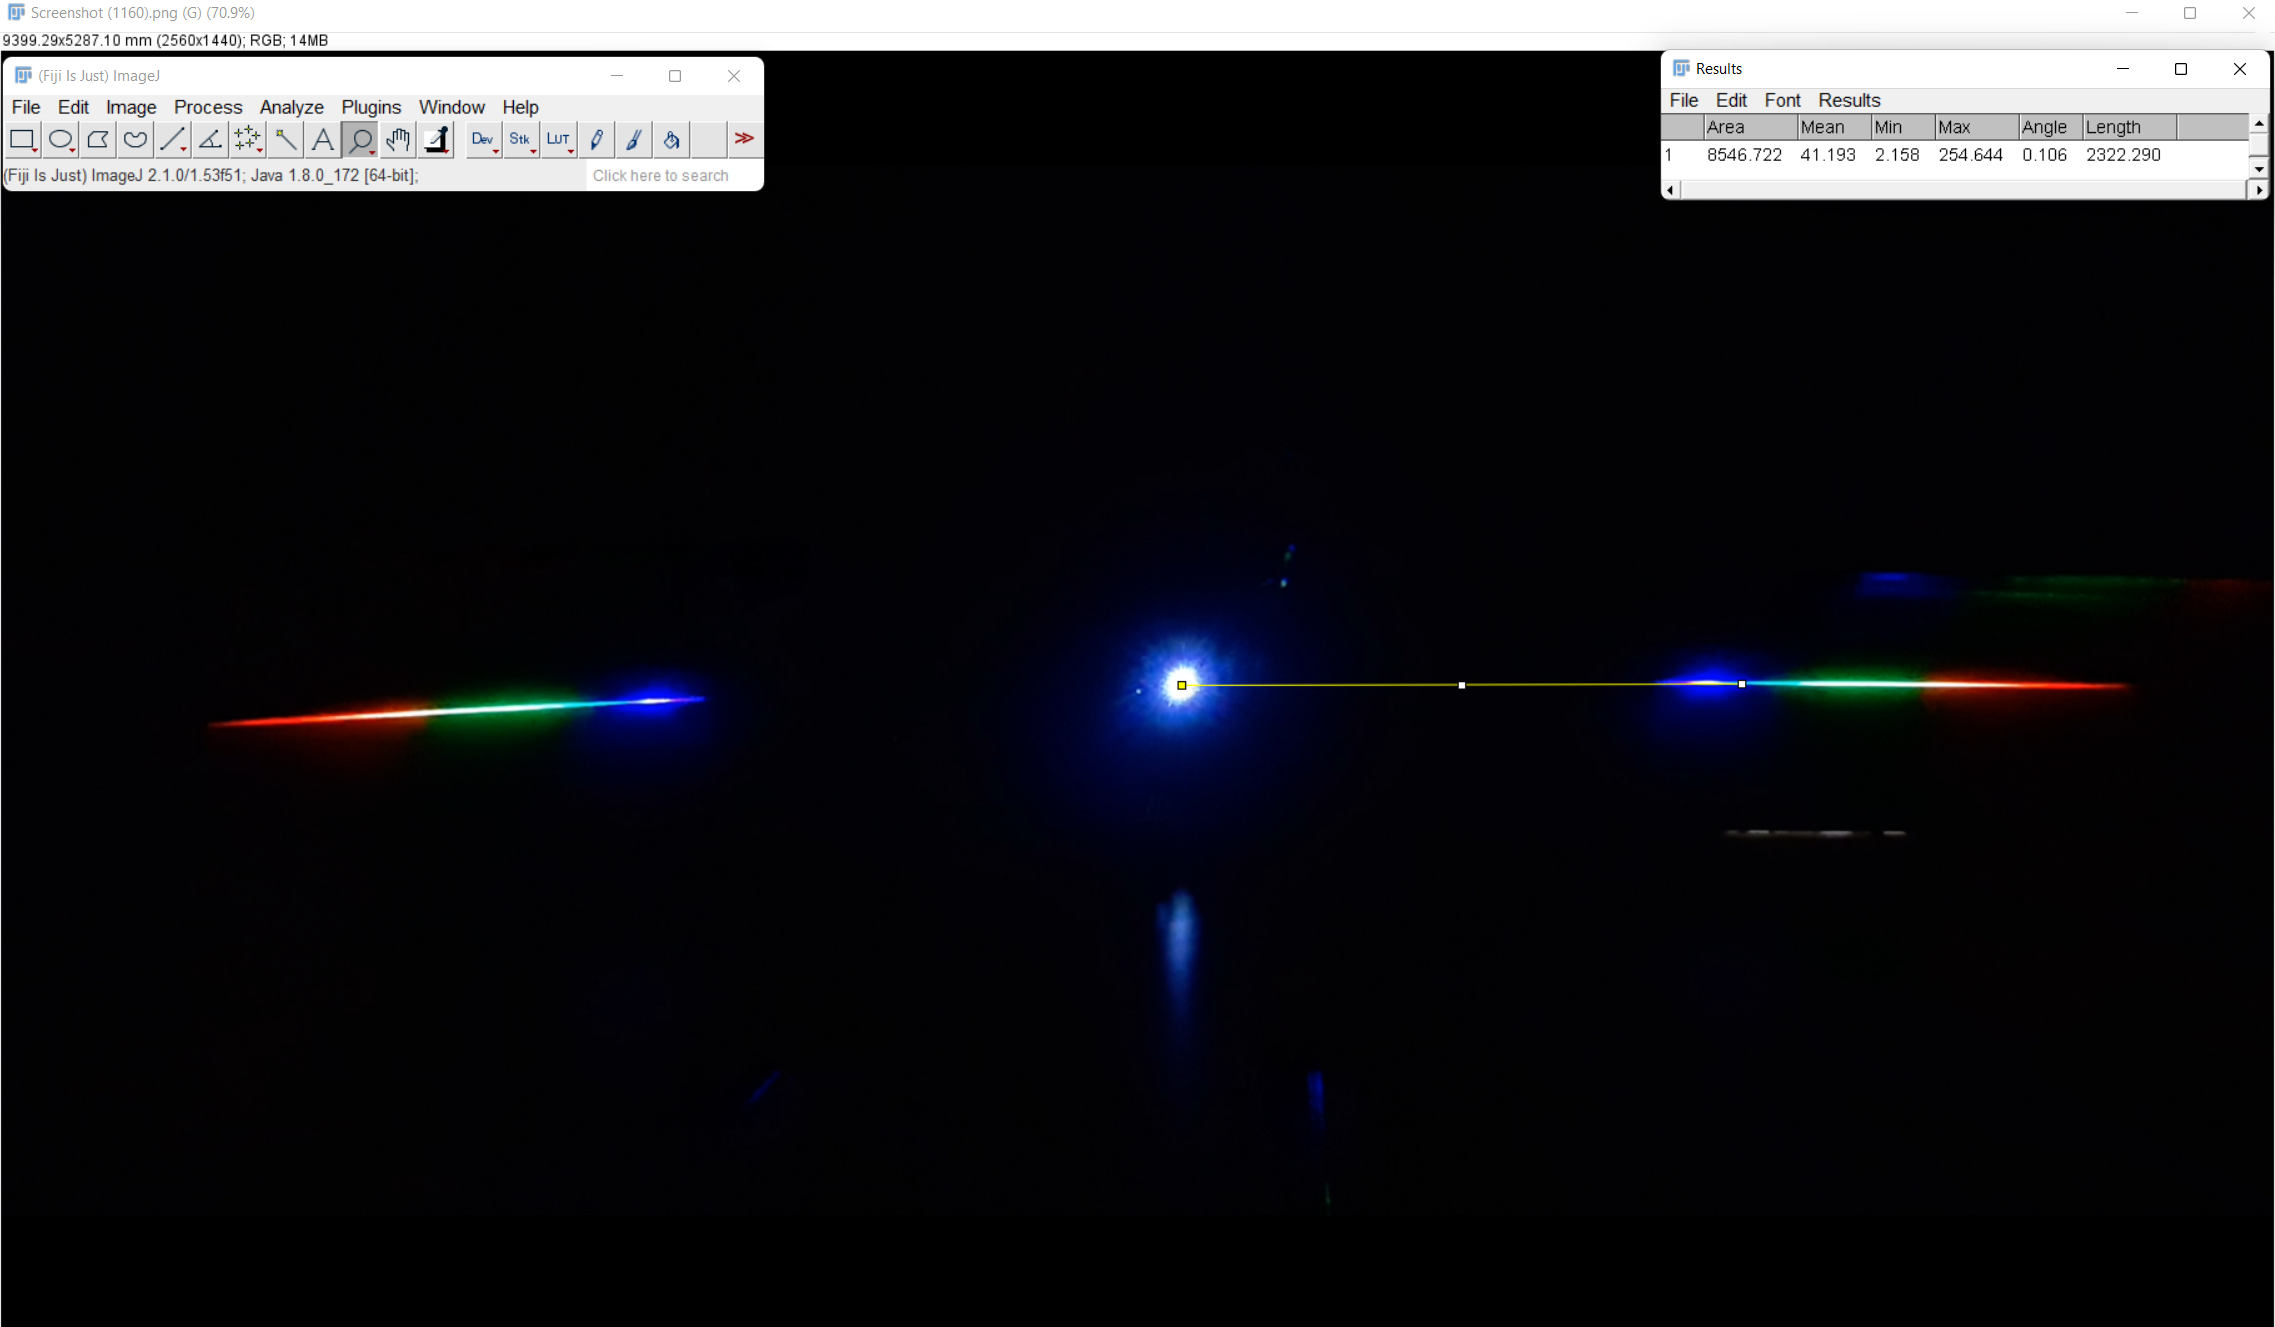
\includegraphics[scale=0.15]{Conclusione/mis.png}
  \caption{In these two images it is possible to visualize the way in which the distances between the real source and the virtual source have been measured.}
\end{figure}